% !TEX root = ../main.tex
\section{Methodology}\label{sec:method}

\subsection{Preprocessing}\label{sec:preprocessing}

% Steps 1-6 of the pipeline figure, one paragraph.
\begin{figure}[t]
  \centering
  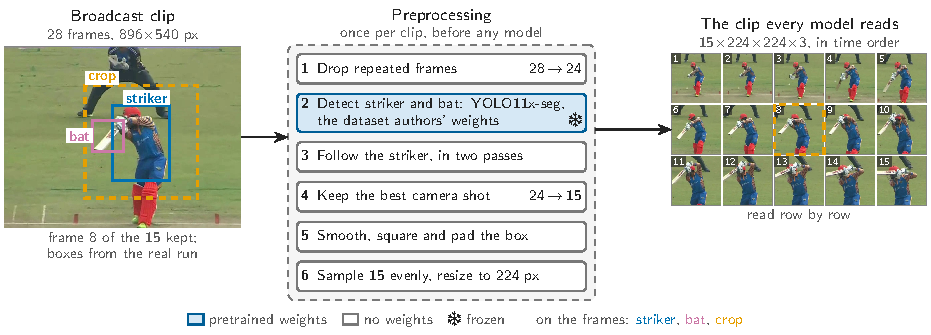
\includegraphics[width=\textwidth,height=0.85\textheight,keepaspectratio]{fig_pipeline.pdf}
  \caption{Preprocessing. Every clip becomes 15 frames of
  224\,$\times$\,224 px centred on the striker. Steps 1--6 run once per clip;
  only step 2 has learned weights, the dataset authors' YOLO11x-seg detector,
  kept frozen. The example is a validation Cover Drive (vid533\_0): 28 broadcast
  frames, 24 after removing repeats, 15 in the camera shot with the most
  detections. The boxes are the ones the pipeline produced on frame 8.}
  \label{fig:pipeline}
\end{figure}

\subsection{Frame models}\label{sec:frame_models}

\begin{figure}[t]
  \centering
  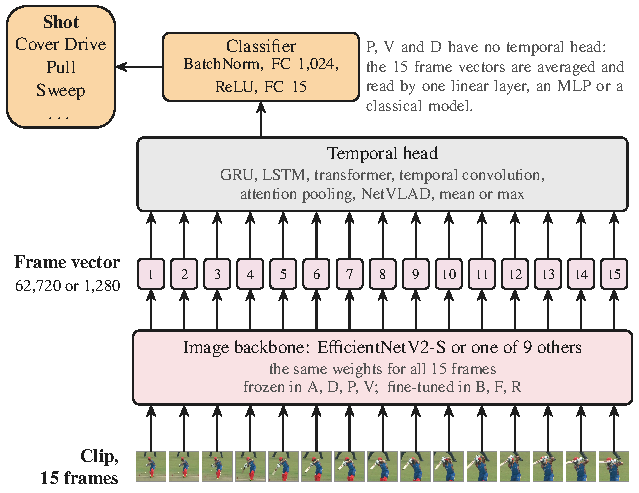
\includegraphics[width=\textwidth,height=0.85\textheight,keepaspectratio]{fig_frame_models.pdf}
  \caption{Frame models. One image backbone turns each of the 15 frames into a
  vector, a temporal head reads the 15 vectors, and a classifier scores the 15
  shots. The backbones are listed in Table~\ref{tab:image_backbones} and the
  heads in Table~\ref{tab:temporal_heads}.}
  \label{fig:frame_models}
\end{figure}

% The options behind the architecture figures, with the experiments that use
% them. Needs \usepackage{booktabs}. \input this file where the tables belong,
% or paste the tables in: Springer wants a single .tex file at submission.

\begin{table}[ht]
\centering
\caption{Image backbones of the frame models (Fig.~\ref{fig:frame_models}),
and how each one was used. A frozen backbone runs once and its frame vectors
are stored; a fine-tuned one trains with the head.}
\label{tab:image_backbones}
\begin{tabular}{@{}lll@{}}
\toprule
Backbone & Frozen & Fine-tuned end to end \\
\midrule
\multicolumn{3}{@{}l}{\textit{CNNs, pretrained on ImageNet}} \\
EfficientNetV2-S  & A01--A14, D01--D06, P01 & B01, F01--F05, R01--R03 \\
EfficientNetV2-B3 & -- & B02 \\
Xception          & -- & B03 \\
ConvNeXt-T        & P02 & B04 \\
MobileNetV3-L     & -- & B05 \\
ResNet-50         & -- & B06 \\
RegNetY-16GF      & -- & B07 \\
\multicolumn{3}{@{}l}{\textit{Vision transformers}} \\
Swin-T, ImageNet  & -- & B08 \\
CLIP ViT-B/16$^{a}$ & P05, V09 & -- \\
DINOv2-B$^{b}$ & V10 & -- \\
\bottomrule
\end{tabular}
\par\vspace{2pt}{\footnotesize $^{a}$ trained on 400\,M image--text pairs;\quad
$^{b}$ self-supervised, no labels.}
\end{table}

\begin{table}[ht]
\centering
\caption{Temporal heads of the frame models, grouped by how they treat the
order of the 15 frames. Each is followed by the same classifier: BatchNorm,
FC 1,024 with ReLU, FC 15.}
\label{tab:temporal_heads}
\begin{tabular}{@{}ll@{}}
\toprule
Temporal head & Experiments \\
\midrule
\multicolumn{2}{@{}l}{\textit{Recurrent: read the frames in order}} \\
GRU-128, last state & A03, B01--B08, R01--R03 \\
GRU-64 / BiGRU-128 & A04 / A05 \\
LSTM-64 / BiLSTM-64 & A06 / A07 \\
GRU-128 after a LayerNorm & A13 \\
GRU-128 on averaged feature maps & A14 \\
GRU-128 with attention over its steps & F05 \\
\multicolumn{2}{@{}l}{\textit{Attention: each frame attends to all 15}} \\
Transformer, 2 layers, 4 heads & A08, F02 \\
Transformer, 4 layers, 8 heads & A09 \\
\multicolumn{2}{@{}l}{\textit{Convolution over time}} \\
Dilated temporal convolution, rates 1, 2, 4 & A10 \\
\multicolumn{2}{@{}l}{\textit{Pooling: frame order ignored}} \\
Mean / max over frames & A01 / A02 \\
Attention pooling & A11 \\
NetVLAD, 8 learned centres & A12 \\
\multicolumn{2}{@{}l}{\textit{No temporal head: the frame vectors averaged}} \\
One linear layer (a probe) & P01, P02, P05 \\
MLP, 1,024 hidden & V09, V10 \\
Logistic regression, RBF SVM, random forest, & D01--D06 \\
\quad XGBoost, 10-NN, MLP & \\
\bottomrule
\end{tabular}
\end{table}

\begin{table}[ht]
\centering
\caption{Video backbones (Fig.~\ref{fig:video_models}a), the input each one
takes, and how it was used. Our 15 frames become 16 by repeating the middle
one and 8 by keeping every other one.}
\label{tab:video_backbones}
\begin{tabular}{@{}lccccc@{}}
\toprule
Backbone & Frames & Size (px) & Fine-tuned, & Frozen, & Frozen, \\
 & & & new linear & MLP & one linear \\
\midrule
\multicolumn{6}{@{}l}{\textit{3D CNNs, Kinetics-400}} \\
R3D-18 & 15 & 112 & C02 & V01 & P03 \\
MC3-18 & 15 & 112 & -- & V02 & -- \\
R(2+1)D-18 & 15 & 112 & C01 & V03 & -- \\
S3D & 15 & 224 & -- & V04 & -- \\
I3D-R50 & 8 & 224 & C03 & -- & -- \\
SlowFast-R50 & 32 + 8$^{a}$ & 224 & C04 & -- & -- \\
X3D-M & 16 & 224 & C05 & -- & -- \\
\multicolumn{6}{@{}l}{\textit{Video transformers, Kinetics-400}} \\
MViTv2-S & 16 & 224 & C06 & V06 & -- \\
Swin3D-T & 15 & 224 & C07 & V05 & -- \\
VideoMAE-B & 16 & 224 & C08 & V07 & P04 \\
TimeSformer-B & 8 & 224 & -- & V08 & -- \\
\bottomrule
\end{tabular}
\par\vspace{2pt}{\footnotesize $^{a}$ SlowFast reads the clip twice: 32 frames on its fast path, 8 on its slow one.}
\end{table}


\subsection{Video models}\label{sec:video_models}

\begin{figure}[t]
  \centering
  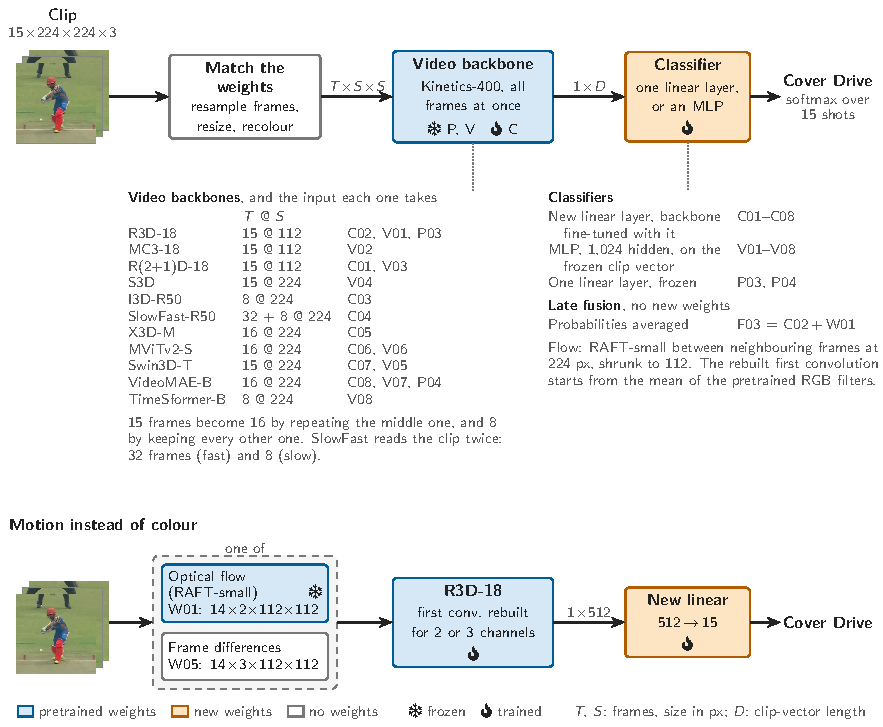
\includegraphics[width=\textwidth,height=0.85\textheight,keepaspectratio]{fig_video_models.pdf}
  \caption{Video models. (a)~The clip is resampled to the input its
  Kinetics-400 weights expect, and the backbone reads space and time together
  (Table~\ref{tab:video_backbones}). (b)~R3D-18 reads motion instead of colour:
  optical flow from RAFT-small (W01) or frame differences (W05). The tiles are
  the real flow fields and differences of the example clip.}
  \label{fig:video_models}
\end{figure}

\subsection{Pose and bat tracks}\label{sec:pose}

\begin{figure}[t]
  \centering
  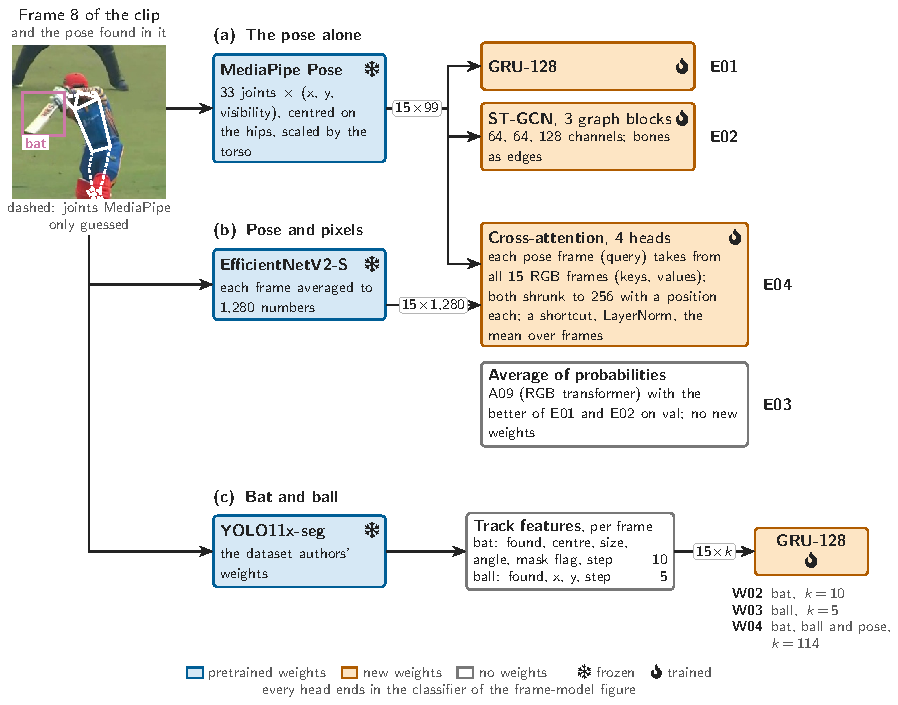
\includegraphics[width=\textwidth,height=0.85\textheight,keepaspectratio]{fig_pose_tracks.pdf}
  \caption{The batter's body and the bat instead of pixels. (a)~MediaPipe's 33
  joints per frame, read by a GRU (E01) or a graph network whose edges are the
  bones (E02). (b)~E04: each pose frame takes what it needs from the RGB frames
  through cross-attention. (c)~W02--W04: the bat and ball tracks from the
  dataset authors' detector. Every extractor is frozen; only the heads train.
  The skeletons and bat boxes are the ones the models read.}
  \label{fig:pose}
\end{figure}

\subsection{The multi-scale hybrid (F02)}\label{sec:f02}

\begin{figure}[t]
  \centering
  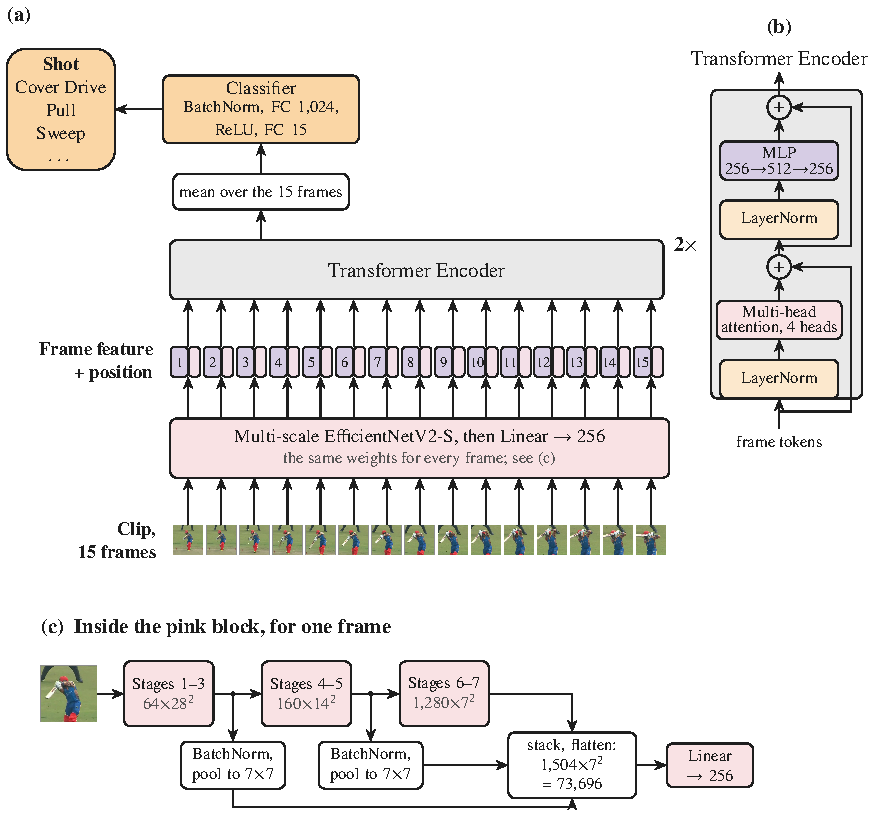
\includegraphics[width=\textwidth,height=0.85\textheight,keepaspectratio]{fig_f02.pdf}
  \caption{F02, the multi-scale hybrid. (a)~Each frame passes through the same
  multi-scale EfficientNetV2-S and a linear layer; a learned position is added;
  two transformer encoder layers mix the 15 frames, and their mean goes to the
  classifier. (b)~One encoder layer. (c)~Inside the frame encoder: the maps
  after stages 3 and 5 are normalised, pooled to the last 7\,$\times$\,7 grid
  and stacked with it. 40.4\,M weights, half of them new. F01 is the same
  encoder under GRU-128.}
  \label{fig:f02}
\end{figure}

\subsection{Final ensemble}\label{sec:ensemble}

\begin{figure}[t]
  \centering
  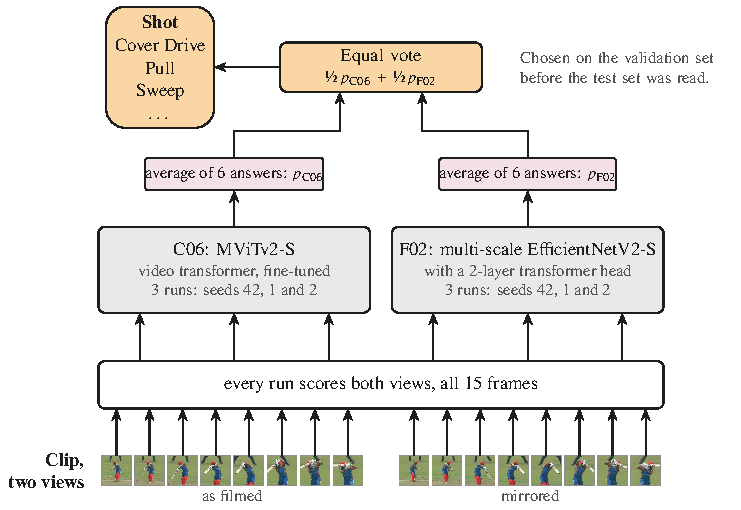
\includegraphics[width=\textwidth,height=0.85\textheight,keepaspectratio]{fig_ensemble.pdf}
  \caption{The final system, chosen on the validation set before the test set
  was read. The three runs of C06 and of F02 score the clip as filmed and
  mirrored; each model's six answers are averaged, and the two models vote with
  equal weight.}
  \label{fig:ensemble}
\end{figure}

\subsection{Training and implementation}\label{sec:training}

% Optimiser, schedule, augmentation, label smoothing, seeds, hardware (Arc B580 / CUDA).
